\documentclass[english]{article}
\usepackage[T1]{fontenc}
\usepackage[utf8]{luainputenc}
\usepackage{graphicx}
\usepackage{babel}
\usepackage{xcolor}
%Gummi|065|=)
\title{\textbf{RPC DAQ based on DIM}}
\author{L.Mirabito}
\date{}
\begin{document}

\maketitle

\section{Architecture}

\subsection{PC names and role}
Usually the acquisition is based on RaspberryPI micro computers controlling and reading each the 12 DIFs connected 4 planes each. Data are collected and written to disk on a separate linux PC .

The  RPIs are responsible for chip configurations, DIF control and data readout. One RPI is also handling the control of the SDCC (Detector clock \& command Card) . The central PC is in charged of the configuration database access, the data collection, the event building and writing and the human interface instance

Since DIM is the network framework used in this data acquisition, the DIM DNS must be started on the central PC  with:

\begin{verbatim}
killall -9 dns
export DIM_DNS_NODE=lyopc520
/opt/dhcal/dim/linux/bin/dns &>/dev/null &
\end{verbatim}

\subsubsection{ Standalone PC}

If the single DIF setup is used, the two USB ports of the DIF are used and the SDCC is emulated in the DIF FPGA.
The USB2 port (mezzanine one) corresponds to the usual DIF port, the on-board one is the SDCC port. 

\subsection{DIF control}

On each RPI should run a DIM daemon that controls the DIF connected to it. It is started with

{\sl \bf sudo /etc/init.d/dimdifd start }

its status is obtained with 

{\sl \bf sudo /etc/init.d/dimdifd status }

and it can be stoped with

{\sl \bf sudo /etc/init.d/dimdifd stop }

The log file is {\sl \bf /var/log/dimdif.log }

It is a DIM server acknowledging the following commands:
\begin{itemize}
\item { \bf SCANDEVICES }: List all DIFs connected on USB and publish a DIM Service DEVICES of 255 integers with the identifiers of the found DIFs
\item {\bf INITIALISE}: requires the DIF identifier, it opens the DIF devices and tries to write and read the test register. It updates the Dim Services STATE and INFO and returns an INITIALISED state in case of success or INIT\_FAILED
\item {\bf REGISTERSTATE}: requires the control register (integer) and the current Database state (string). It stores the control register to be used at the next configuration and subscribes to the database DIM server services publishing DIF parameters for each DIF separately (/DB/{\sl STATE\_NAME}/DIF{\sl id}). By this way it obtains from the dimdb service the configuration parameter of each DIF.

\item {\bf CONFIGURE}: it configures all connected DIF and their asoociated ASICs. It updates the STATE and the INFO of each DIF. The STATE contains the whole decoding of the slow control status. 


\item {\bf START}: it starts the acquisition of each DIF. The STATE of each DIF is updated to STARTED.

\item {\bf STOP}: it stops the acquisition of each DIF. The STATE of each DIF is updated to STOPPED.

\end{itemize}

It also publishes 3 services per DIF:
\begin{itemize}
\item {\bf STATE}: a string containing the current DIF state (FOUND, INITIALISED, PRECONFIGURED, CONFIGURED, STARTED, STOPPED)

\item {\bf INFO}: a structure with {\sl dif id, status, slow control status, bcid, gtc,  bytes read and pc name}

\item {\bf DATA}: the last DIF data buffer read. 
\end{itemize}

\subsubsection{Possible issue}

On INITIALISE the USB access may have changed (micro power cut), in this case the daemon exits and dies (open failed in the log).  It has to be restarted.

\subsection{SDCC control}

A DIM daemon is running on the RPI (or single PC) where the SDCC is connected.It is started with

{\sl \bf sudo /etc/init.d/dimcccd start }

its status is obtained with 

{\sl \bf sudo /etc/init.d/dimcccd status }

and it can be stoped with

{\sl \bf sudo /etc/init.d/dimcccd stop }
 
 The log file is {\sl \bf /var/log/dimccc.log }
 
 It acknowlegdes the following commands:
 \begin{itemize}
\item {\bf INITIALISE}: requires the CCC FTDI identifier ("DCCCCC01"), it opens the SDCC devices and tries to write and read the test register. 
\item {\bf CONFIGURE}: it sends DIFRESET and CCCRESET before the start of the acquisition
\item {\bf DIFRESET}: it sends a DIFRESET command on the DCC bus
\item {\bf CCCRESET}: it send a CCCRESET command on the DCC bus
\item {\bf PAUSE}: it send a PAUSE command on the DCC bus
\item {\bf RESUME}: it send a RESUME command on the DCC bus
\item {\bf START}: it send a START\_ACQUISITION command on the DCC bus
\item {\bf STOP}: it send a STOP\_ACQUISITION command on the DCC bus
\item { \bf TESTREGISTERREAD }: read the test register and update the REGISTER DIM service
\item { \bf TESTREGISTERWRITE }: requires an integer value that is written in the test register
\end{itemize}

It publishes 2 DIM services, {\bf REGISTER} that is filled when TESTREGISTERREAD is called and an integer {\bf STATUS} which value is changed depending on the last command received.
 
\subsubsection{Possible issue}

At power on, the USB control may be faulty. It is recommended to INITIALISE and use the TESTREGISTERWRITE/READ to check the correct access of the FPGA.

\subsection{Database control}

The database control is the responsability of one DIM daemon server running on the central PC. It is started with

{\sl \bf sudo /etc/init.d/dimdbd start }

its status is obtained with 

{\sl \bf sudo /etc/init.d/dimdbd status }

and it can be stoped with

{\sl \bf sudo /etc/init.d/dimdbd stop }
 
 The log file is {\sl \bf /var/log/dimdb.log }
 
 It acknowlegdes the following commands:
 \begin{itemize}
\item {\bf DOWNLOAD}: requires the name of the needed DB state ("LPCC\_230"), it downloads the given state from the configuration databas and creates for each DIF a DIM service withe name /DB/{\sl STATE\_NAME}/DIF{\sl id} containing the configuration parameters for all the ASICs of the given DIF 
\item {\bf DELETE}: it deletes all the DIM services of the current state
\item {\bf NEWRUN}: it asks the database for a new run number and update /DB/RUNFROMDB service

\end{itemize}

\subsection {Data writing}

The data writing is achieved by one DIM daemon server running on the central PC. It is started with

{\sl \bf sudo /etc/init.d/dimwriterd start }

its status is obtained with 

{\sl \bf sudo /etc/init.d/dimwriterd status }

and it can be stoped with

{\sl \bf sudo /etc/init.d/dimwriterd stop }
 
 The log file is {\sl \bf /var/log/dimwriter.log }
 
 It acknowlegdes the following commands:
 \begin{itemize}
\item {\bf INITIALISE}: it subscribes to all possible DIF DATA and INFO services connected to the DIM DNS. It also subscribes to the RUNFROMDB service from the dimdb server. It creates an {\sl ShmProxy} instance that is spying the {\sl /dev/shm} directory for new data collected. The {\sl infoHandler} method of the server received data from the {\sl dimdif} daemon DATA services and write them in {\sl /dev/shm}
\item {\bf START}: it opens an LCIO file in {\sl /data/online/Results} using the current value of run obtained by the RUNFROMDB service. It starts the {\sl /dev/shm} spying, collects data and writes them to disk when all publishing DIF have completed the same BCID buffer.
\item {\bf STOP}: it stops the spying and closes the data file.
\end{itemize}

\subsubsection{Possible issue}

This server is still partially in development. In case of failure (no data writen, crash) one should stop the run, restart this daemon only, re-initialise it and restart a run. There is no need to restart the whole DAQ

\section {DAQ control}


\subsection{ The DimDaqControl package }
The control of the DAQ is done via { \bf \sl DimDaqControl } a standalone DIM program interfaced to python. The python package LSDHCALDimCtrl  is in {\sl /home/acqilc/SDHCAL/DimCtrl}. The environment needs to be set properly with:

\begin{verbatim}
cd /home/acqilc/SDHCAL/DimCtrl
export LD_LIBRARY_PATH=.:./lib:$LD_LIBRARY_PATH
python
\end{verbatim}  

Inside the python shell launched you can do the following:

\begin{enumerate} 
\item \textcolor{red}{ \bf  import LSDHCALDimCtrl} :  imports the python package

\item \textcolor{red}{\it \bf s=LSDHCALDimCtrl.DimDaqControl("Tomuvol")}:  creates an instance of DimDaqControl

\item \textcolor{red}{\it \bf s.scandns()}: lists all DIMServer, services and commands available on the DIM DNS  
\item \textcolor{red}{\it \bf s.initialiseWriter("/data/online/Results")}: Initialise the data writing on the given directory. It has to be done only once if the dimwriter daemon is not stopped.

\item \textcolor{blue}{\it \bf s.scan()}: sends a SCANDEVICES command to all dimdif servers and wait for DEVICES service update. It must be called once or after a destroy()


\item \textcolor{blue}{\it {\bf s.initialise()}}: sends an INITIALISE command to all DIF found previously
\item {\bf s.\_print()}: prints the status of each DIF on each dimdif server from the INFO service of each given DIF. Like the scan() command it must be called only after a scan() command

\item {\bf s.download("LPCC\_230")}: triggers the DELETE of the previous state in the DB server and the DOWNLOAD of the specified state. Since no semaphore mechanism is used in this command a 20 s delay may be needed before the data are available. It has to be called only when a new DB state needs to be downloaded or when the dimdb daemon is restarted

\item \textcolor{purple}{\bf s.registerstate(0x815A1B00,"LPCC\_230")}: send a REGISTERSTATE command to all dimdif server. The state specified should be identical to the last downloaded state in dimdb. It must be called before configure to also set the control register.

\item \textcolor{purple}{\bf s.configure()}: sends a CONFIGURE command to all dimdif servers




\item \textcolor{green}{\bf s.start()}: starts a run, sends a START command to the dimccc, the dimdif and the dimwriter servers 

\item \textcolor{green}{\bf s.stop()}: stops a run,sends a STOP command to the dimccc, the dimdif and the dimwriter servers
\item \textcolor{blue}{\bf s.destroy()}: send a DESTROY command to the dimdif servers. All the DIF handling are cleared locally so the only possible next command is scan()
\end{enumerate} 

The red commands needs to be used only once per session. The blue ones should be used once or if any changes has occurred on dimdif servers (power cycle for example). The purple ones are used to reconfigure chips. The green ones are the normal one to start and stop a run. Eventually the black commands are optional, the {\bf download} one must be called at least ones to access the DB but is not needed in a new session if the dimdb server is alive and already contains the state 
\subsection{Spying with webDid}
The latest versions of DIM provide a web interface to all DIM servers and clients. The server is started with:
\begin{verbatim}
export DIM_DNS_NODE=lyopc520
export LD_LIBRARY_PATH=/opt/dhcal/dim/linux:$LD_LIBRARY_PATH
/opt/dhcal/dim/WebDID/webDid
\end{verbatim}

Then the interface can be accessed via a web browser at address http://lyopc520:2500 as seen on figure \ref{webdid}
\begin{figure}[htp]
\centering
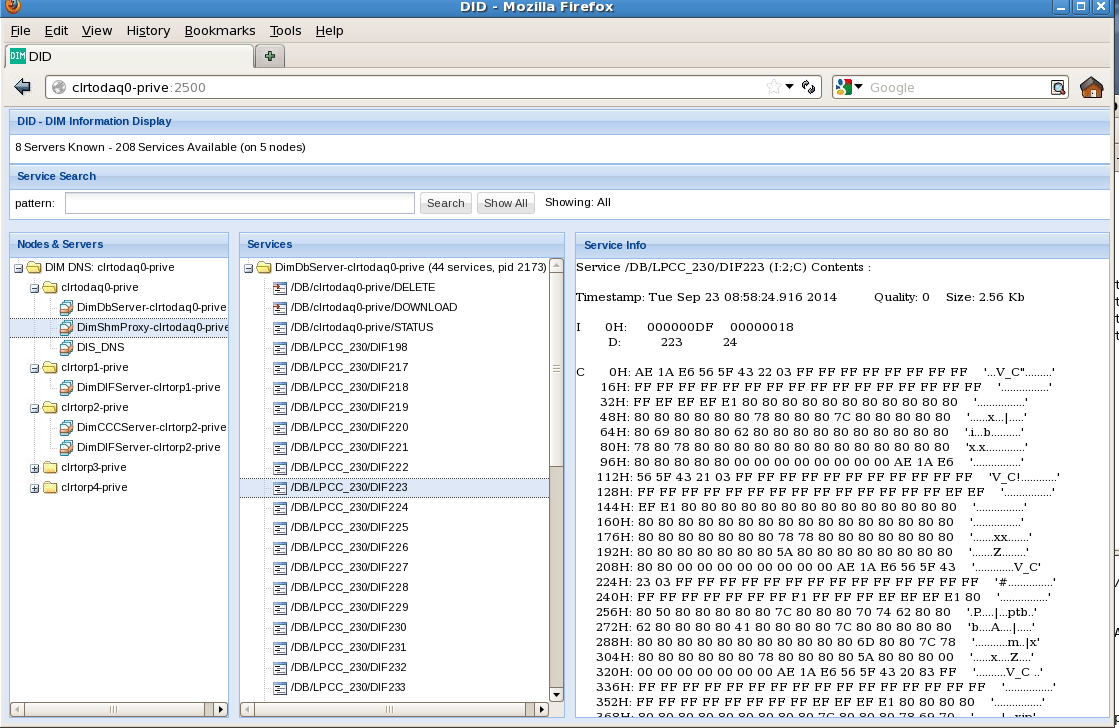
\includegraphics[width=1.3\textwidth]{./webDid.png}
\caption{The web application webDID used to spy DIM services}
\label{webdid}
\end{figure}

Commands can be sent manually but spying of dynamically allocated infos (like the DID DATA service) should be avoided since it crashes the program. 
\subsection{Other tips}
\subsubsection{Restarting the whole daq}
In case of problem, after exiting the python shell, one can possibly restart the dns and launch
\begin{verbatim}
source ~/restartdimdaq
\end{verbatim}
It restarts all needed daemons

\section{Changing configuration Database}

The python package to be used is in {\bf /data/online/python/OracleAccess.py} on the central PC.
The following commands are an example of its typical usage:
\begin{itemize}
\item \textcolor{blue}{\bf import OracleAccess as oa} : imports the DB package
\item \textcolor{blue}{\bf help(oa)}: prints an help on all possible commands
\item \textcolor{blue}{\bf s=oa.OracleAccess("DIF174\_24HR\_AllInOne")} : creates an access  to the state {\sl DIF174\_24HR\_AllInOne }
\item \textcolor{blue}{\bf s.toXML()}: dumps all the parameters of the current state to {\sl DIF174\_24HR\_AllInOne.xml }

\item \textcolor{blue}{\bf s.ChangeThreshold(190,500,300)}: Changes the thresholds on all ASICs to B0=190,B1=500, B2=300
\item \textcolor{blue}{\bf s.uploadChanges()}: Creates a new state  {\sl DIF174\_24HR\_AllInOne\_1 } with the new thresholds

\item \textcolor{blue}{\bf s.dumpStateNames()}: Dumps all states names in the DB

\end{itemize}

Typically gains, masks and thresholds are changed, please contact the author if changes on other parameters are required

 
\end{document}


